\documentclass[11pt,a4paper]{article}
\usepackage[margin=2.3cm]{geometry}
\usepackage{amsmath,amssymb}
\usepackage{graphicx}
\usepackage{booktabs}
\usepackage[hidelinks]{hyperref}
\usepackage{microtype}
\graphicspath{{../figures/}}
\setlength{\parskip}{0.45em}
\setlength{\parindent}{0pt}

\title{Adaptive TMUA practice from a small, cold-start question bank:\\ a simulation study of Kevinvariant Smart Practice}
\author{Kevin Hu}
\date{October 2026}

\begin{document}
\maketitle

\begin{abstract}
Smart Practice is an adaptive practice mode on Kevinvariant, my free TMUA preparation website. It uses item response theory (IRT), the standard method behind adaptive tests such as the GMAT; the method is not new. What is unusual is the setting: 440 original questions, no response data at launch, and a static website with no server of its own. Before any real data exist, I tested the system by simulation. Calibration recovers question difficulty steadily as answers accumulate, and never does worse than the author's ratings it starts from (difficulty error 0.40 with ratings alone, 0.21 at about 145 answers per question). Adaptive selection reaches a standard error of 0.4 on the ability scale (about 0.8 TMUA points) after 11 questions, against 30 for random selection, once the questions are calibrated; on launch day, with ratings only, it needs 23 against more than 30.
\end{abstract}

\section{The system}

\paragraph{Model.} Each question $i$ has a difficulty $b_i$ and a discrimination $a_i$. A student of ability $\theta$ answers it correctly with probability
\begin{equation}
P_i(\theta) = c_i + (1-c_i)\,\frac{1}{1+e^{-a_i(\theta-b_i)}}, \qquad c_i = \frac{1}{k_i},
\end{equation}
where $k_i$ is the number of options. The guessing floor $c_i$ is fixed rather than estimated, because the TMUA has no negative marking and blind guessing pays exactly $1/k_i$; estimating it from small samples is notoriously unstable.

\paragraph{Scale and priors.} The ability scale is anchored to the TMUA: $\theta = 0$ is the median candidate and $\theta = 1$ one candidate standard deviation, so that a TMUA score is roughly $S = 4.5 + 1.951\,\theta$. This uses the published anchoring of the 1.0 to 9.0 scale (median 4.5, 90th percentile 7.0) and a logistic slope of 0.68 per TMUA point fitted earlier to published raw-mark anchors. Every question on the site already has a difficulty rating $r_i$ on the same scale, which gives the priors
\begin{equation}
b_i \sim \mathcal{N}\!\left(\frac{r_i - 4.5}{1.951},\ 0.384^2\right), \qquad \log a_i \sim \mathcal{N}\!\left(\log 1.327,\ 0.3^2\right),
\end{equation}
where 0.384 corresponds to a rating being off by 0.75 TMUA points.

\paragraph{Calibration.} Each week, anonymous answers that students chose to share are fitted by Bayes-modal marginal maximum likelihood (the Bock--Aitkin EM algorithm with the priors above). Each student's ability is integrated over a 41-point grid rather than estimated, which keeps students with only a few answers from distorting the questions, and the site's population is modelled as $\mathcal{N}(\mu, \sigma^2)$ with both parameters estimated. With fewer than 3000 usable answers or a median below 50 per question, discrimination is fixed for all questions (a 1PL fit).

\paragraph{Adaptive practice.} In the browser, ability is the posterior mean (EAP) on a 71-point grid. The next question maximises Fisher information
\begin{equation}
I_i(\theta) = \frac{\left[a_i (1-c_i)\, s(1-s)\right]^2}{P_i(\theta)\,(1-P_i(\theta))}, \qquad s = \frac{1}{1+e^{-a_i(\theta-b_i)}},
\end{equation}
subject to three practical rules: topics rotate (no topic twice running, shares tracking the bank), one of the five most informative questions is picked at random so the same questions are not always shown, and every fifth question, or after two misses, is an easier one with a 70 to 90 percent chance of success.

\section{Simulation design}

The truth is drawn from the priors themselves: each question's true difficulty is its rating-based prior plus $\mathcal{N}(0, 0.384^2)$ noise, and its true discrimination is log-normal around 1.327. The real bank of 440 questions is used, with their real option counts. Simulated students have $\theta \sim \mathcal{N}(0.8, 0.9^2)$, stronger than the median TMUA candidate, as one would expect of students on a preparation site. The production code is used throughout: the Python calibration and the JavaScript engine that runs in the browser.

\textbf{(a) Recovery.} Between 25 and 3200 students each answer 20 questions drawn at random from the whole bank (1 to 145 answers per question), five replications per size, fitted as 2PL and 1PL.

\textbf{(b) Adaptive versus random.} 1000 students each answer 30 questions chosen by Smart Practice as shipped, by pure maximum information, or at random. The engine either knows the true parameters (``calibrated'') or only the rating-based priors (``ratings only'', as on launch day). Answers always come from the true parameters.

\section{Results}

\begin{figure}[h]
\centering
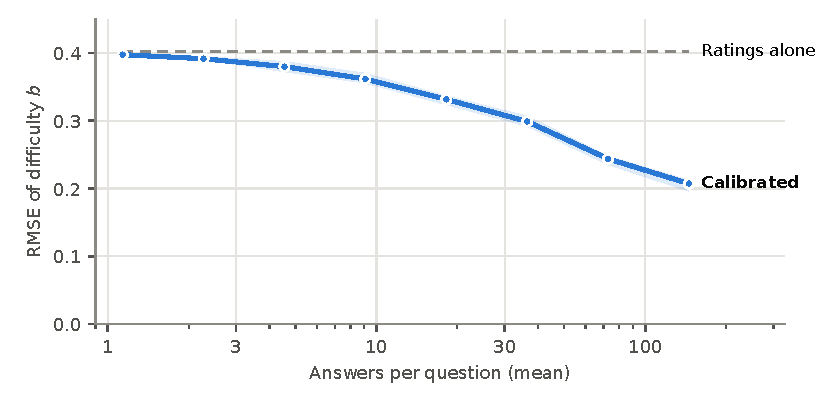
\includegraphics[width=0.82\textwidth]{recovery_b.pdf}
\caption{Error in question difficulty against the mean number of answers per question (log scale). Line: mean of five replications; band: their range. Dashed: the error of the ratings alone.}
\label{fig:b}
\end{figure}

\paragraph{Difficulty is recovered steadily (Figure~\ref{fig:b}).} The root mean square error of $b$ falls from 0.40 with ratings alone to 0.33 at 18 answers per question, 0.24 at 73 and 0.21 at 145. Because the ratings act as priors, sparse data never make the estimates worse than the ratings. The 1PL fit is within 0.01 of the 2PL fit for difficulty at every size, so only 2PL is drawn. Population mean and spread are recovered at 0.82 to 0.85 and 0.79 to 0.87 for 100 or more students (true 0.8 and 0.9).

\paragraph{Discrimination needs far more data.} Its error falls only from 0.44 to 0.37 at 73 answers per question and 0.33 at 145. This supports the rule of fixing discrimination until the data are large.

\paragraph{Uncertainty is mostly honest.} The share of true difficulties inside the reported 95 percent intervals is 0.93 to 0.94 up to 800 students and 0.91 at 3200: slightly overconfident with a lot of data.

\begin{figure}[h]
\centering
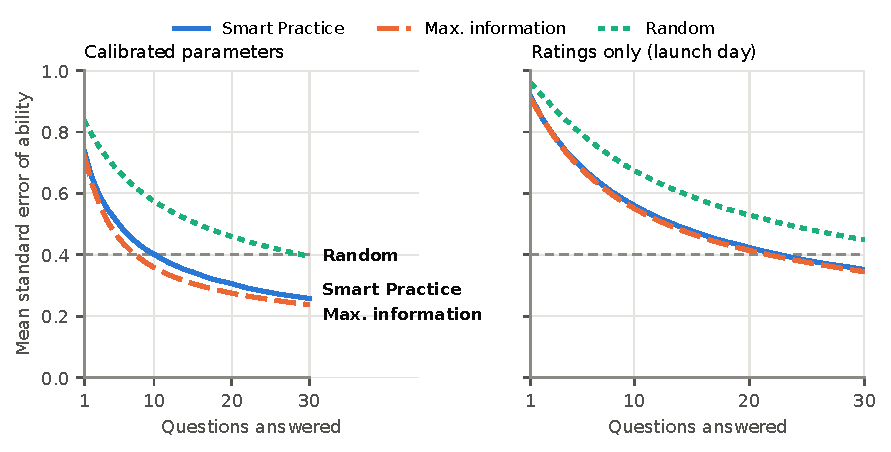
\includegraphics[width=0.9\textwidth]{cat_se.pdf}
\caption{Mean standard error of the ability estimate after each question, whole bank. Dashed line: 0.4, about 0.8 TMUA points. Left: the engine knows the calibrated parameters. Right: ratings only.}
\label{fig:cat}
\end{figure}

\begin{table}[h]
\centering
\begin{tabular}{llccc}
\toprule
Questions available & Parameters & Smart Practice & Max.\ information & Random \\
\midrule
All 440 & calibrated & 6 / 11 & 5 / 8 & 16 / 30 \\
All 440 & ratings only & 14 / 23 & 13 / 22 & 24 / $>$30 \\
Free 120 & calibrated & 7 / 13 & 5 / 10 & 14 / 25 \\
Free 120 & ratings only & 14 / 23 & 13 / 22 & 19 / $>$30 \\
\bottomrule
\end{tabular}
\caption{Questions needed for the mean standard error to reach 0.5 / 0.4.}
\label{tab:cat}
\end{table}

\paragraph{Adaptive selection is much faster (Figure~\ref{fig:cat}, Table~\ref{tab:cat}).} With calibrated questions, Smart Practice reaches a standard error of 0.4 in 11 questions, compared with 30 for random selection; after 10 questions its standard error is 0.40 against 0.57. The practical rules cost about three questions against pure maximum information, a fair price for variety and for not always showing the same questions. With ratings only, the advantage shrinks (23 against more than 30) because the engine's picture of each question is blurred, which is exactly what calibration fixes. The free pool of 120 questions behaves almost as well as the full bank.

\paragraph{The reported range can be trusted once calibrated.} With calibrated parameters the actual error of the estimate matches the reported standard error (0.41 against 0.40 after 10 questions). With ratings only the actual error is about 10 percent larger (0.62 against 0.56), so on launch day the ``likely range'' shown to students is slightly too narrow.

\section{Limitations}

The simulation assumes the model is right, because the truth is drawn from it. Real students will depart from it: questions test more than one skill, Paper 1 and Paper 2 measure somewhat different abilities, and some students guess cleverly rather than blindly. The assumed rating error (0.75 TMUA points) is itself a guess; if the ratings are worse, the priors are overconfident and calibration has more to correct. In part (a) questions were assigned at random, whereas real data will come partly from adaptive sessions, which marginal maximum likelihood handles in principle but which is not tested here. The TMUA figure shown to students rests on external anchors rather than site data, so it is labelled as a rough estimate, never an official prediction. Finally, no real data have been collected yet; the weekly calibration report (which also flags questions whose answers run against ability, a sign of a wrong answer key) will be the real test.

\section{Conclusion}

On a bank of this size, a standard IRT approach with rating-based priors behaves as hoped in simulation: calibration improves steadily on the author's ratings without ever making them worse, and adaptive selection reaches a useful precision in roughly a third as many questions as random practice. The code for the model, the calibration and both simulations is in the site's public repository.

\end{document}
